\documentclass[12pt, titlepage]{article}

\usepackage{amsmath, mathtools}
\usepackage{siunitx}
\usepackage{booktabs}
\usepackage{tabularx}
\usepackage{colortbl}
\usepackage{graphicx}
\usepackage{hyperref}

\hypersetup{
    colorlinks,
    citecolor=blue,
    filecolor=black,
    linkcolor=red,
    urlcolor=blue
}
\usepackage[round]{natbib}

\usepackage{fullpage}

\usepackage{enumitem,amssymb}
\newlist{checklist}{itemize}{2}
\setlist[checklist]{label=$\square$}
\usepackage{pifont}

\begin{document}

\title{System Verification and Validation Plan for Retinal Vessel Segmentation System (RVSS)}
\author{Xinyu Ma}
\date{February 19, 2024}
	
\maketitle

\pagenumbering{roman}

\section{Revision History}

\begin{tabularx}{\textwidth}{p{5cm}p{1.5cm}X}
\toprule {\bf Date} & {\bf Version} & {\bf Notes}\\
\midrule
02/16/2024 & 1.0 & Initial Release  \\
02/19/2024 & 2.0 & Updated based on feedback from the presentation\\ 


\bottomrule
\end{tabularx}

\newpage

\tableofcontents

\listoftables


\newpage

\section{Symbols, Abbreviations and Acronyms}

\renewcommand{\arraystretch}{1.2}
\begin{tabular}{l l} 
  \toprule		
  \textbf{symbol} & \textbf{description}\\
  \midrule 
  CNN & Convolution Neural Network\\
  MG & Module Guide \\
  MIS & Module Interface Specification \\
  SRS & Software Requirement Specification\\
  RVSS & Retinal Vessel Segmentation System \\ 
  TC & Test Case \\
  VnV & Verification and Validation \\ 
  
  \bottomrule
\end{tabular}\\

For complete symbols, abbreviations and acronyms used within the system, please refer the section 1.3 in \href{https://github.com/lele0007/Blood-vessel-segmentation/blob/main/docs/SRS/SRS.pdf}{SRS} document.


\newpage

\pagenumbering{arabic}
This document provides an introductory blurb and roadmap of the Verification and Validation plan for the Retinal Vessel Segmentation System (RVSS). It is designed to ensure that the system meets its specified requirements and fulfills its intended goals effectively (requirements and goals can be found in the \href{https://github.com/lele0007/Blood-vessel-segmentation/blob/main/docs/SRS/SRS.pdf}{SRS} document).The organization of this document starts with the General
Information about the RVSS in \autoref{GeneralInformation}. In  \autoref{plan}, it describes a verification and validation plan.  A system test description is provided in \autoref{systemtests}, which contains tests for functional and nonfunctional requirements. In \autoref{unit_test}, it provides the Unit Test Description.  



\section{General Information}
\label{GeneralInformation}

\subsection{Summary}
This document introduces the validation and verification plan for
the Retinal Vessel Segmentation System (RVSS). The RVSS is a medical imaging application designed to automate the process of segmenting blood vessels from fundus images. It utilizes advanced image processing and machine learning techniques, particularly Convolution Neural Network (CNN), to analyze these fundus images and accurately identify and delineate the blood vessels within the retina.

\subsection{Objectives}
In this section, it states what is intended to be accomplished. The objective is around the qualities that are most important for the RVSS. The following are objectives that are in scope and out of scope.

\begin{itemize}
\item In-Scope Objectives:
\begin{itemize}
\item \textbf{Build Confidence in the Software Correctness}:To ensure that the RVSS operates according to its specifications and user requirements, accurately segmenting blood vessels from fundus images. This involves thorough testing of the segmentation algorithms for sensitivity, recall, and overall accuracy. 
\item \textbf{Ensure the Software Performance}: Focus on verifying the processing speed and responsiveness to ensure that the RVSS can processes fundus images within an acceptable time without sacrificing accuracy.
\end{itemize}

\item Out-of-Scope Objectives:
\begin{itemize}
\item \textbf{Comprehensive Medical Usability Testing}: While comprehensive medical usability testing is valuable, it requires recruiting a large number of participants for fundus photography, which involves user privacy. Due to resource constraints, extensive medical usability testing involving diverse user groups across multiple settings would be out of scope.
\item \textbf{External Libray Verification}: The RVSS relies on external libraries for some of its functionality (e.g., image processing, segmentation algorithms based on machine learning). Given the widespread use and community validation of these external libraries, we can assume that these library has already been verified by its implementation team. Thus, their in-depth verification will be out of scope.

\end{itemize}
\end{itemize}


\subsection{Relevant Documentation}

The relevant documentation for the RVSS includes \href{https://github.com/lele0007/Blood-vessel-segmentation/blob/main/docs/ProblemStatementAndGoals/ProblemStatement.pdf}{Problem Statement} which outlines the specific problem that the RVSS aims to address, \href{https://github.com/lele0007/Blood-vessel-segmentation/blob/main/docs/SRS/SRS.pdf}{System Requirements Specifications} which clearly define the requirements of the system, and design documents, like MG, MIS, etc(found in \href{https://github.com/lele0007/Blood-vessel-segmentation/blob/main/docs}{Github Repository}).  

The problem statement document defines the scope of the problem, the needs of the stakeholders, and the goals that the RVSS seeks to achieve. It guides the development of the verification and validation plan and ensures that the verification and validation processes are aligned with the needs and requirements of the users and stakeholders. The System Requirements Specifications (SRS) document lays out the detailed requirements of the system, including both functional and non-functional requirements. The verification and validation plan directly reference the SRS document to ensure that each specified requirement is implemented correctly in the system. The verification and validation plan refers to design documents (like MG, MIS, etc) to verify that the architecture of the RVSS and each design unit have been correctly realized in the implemented system. 




\section{Plan}
\label{plan}

This section describes the testing plan for the Retinal Vessel Segmentation System (RVSS). It starts with the verification and validation team in section \ref{verification_validation_team}, followed by the SRS verification plan (section \ref{srs_verification_plan}), design verification plan (section \ref{design_verification_plan}), implementation verification plan (section \ref{implementation_verification_plan}), Automated testing and verification tools (section \ref{automated_testing_verification_tools}), and Software validation plan (section \ref{software_validation_plan}).  

\subsection{Verification and Validation Team}
\label{verification_validation_team}

The Verification and Validation Team includes 6 people who plays an important role in ensuring that the developed system meets all specified requirements and is fit for its intended use. The members of Verification and Validation plan is shown in \autoref{verification_validation_member}. 
\newline
\newline

\begin{center}
\begin{table}[h]
\resizebox{\textwidth}{!}{ %
    \begin{tabular}{ |l|p{2cm}|l|p{5cm}| } 
    \hline
    \rowcolor[gray]{0.9}
    \textbf{Name} & \textbf{Role} & \textbf{Document} & \textbf{Responsibilities} \\
    \hline
     Dr.\ Spencer Smith & Instructor/ Reviewer & SRS, VnV plan, MG + MIS & Review all documents. \\ 
     \hline
     Xinyu Ma & Author & SRS, VnV plan, MG + MIS & Create and manage all documents; design, develop and execute test cases. \\  
     \hline
     Kim Ying  Wong& Domain Expert Reviewer-Primary Reviewer & SRS, VnV plan, MG + MIS & Review all documents. \\  
     \hline
     Morteza Mirzaei& Secondary Reviewer & SRS & Review the SRS document. \\
     \hline
    Nada Elmasry& Secondary Reviewer & VnV Plan & Review the VnV plan document. \\ 
    \hline 
    Seyed Ali  Mousavi& Secondary Reviewer & MG + MIS & Review the MG and MIS document. \\
    \hline 
    
    \hline
    \end{tabular} %
}
\caption{Verification and validation team} 
\label{verification_validation_member}
\end{table}
\end{center}

\subsection{SRS Verification Plan}
\label{srs_verification_plan}

The purpose of the SRS Verification Plan is to ensure the SRS document for the RVSS is complete, accurate and meets all necessary standards and requirements. The SRS document shall be verified in the following way: 

\begin{enumerate}

\item  Conduct peer reviews by involving assigned team members (Dr.\ Spencer Smith, Kim Ying Wong, and Morteza Mirzaei) not directly involved in writing the SRS. This helps identify ambiguities, inconsistencies, and missing requirements. For this, the review can be performed referring the following simplified SRS checklist (The checklist refers to the \href{https://github.com/smiths/capTemplate/blob/9251702fdcb9800c59f6ed3d11d91e2bd62fca6d/docs/Checklists/SRS-Checklist.pdf}{SRS checklist} designed by Dr. Smith). 

\textbf{SRS checklist:}
\begin{itemize}
    \item Overall qualities of documentation
      \begin{checklist}
        \item No statement is repeated at the same level of abstraction.
        \item SRS is unambiguous. At least check a representative 
        sample.
        \item SRS is consistent.  At least check a representative sample.
      \end{checklist}
    \item Introduction
      \begin{checklist}
        \item The purpose of the system is clearly defined.
        \item Introductory blurb focuses on the problem domain.
        \item The characteristics of the intended readers and reading suggestions are included and unambiguous.
      \end{checklist}
    \item General System Description
      \begin{checklist}
        \item System context includes a figure showing the relation between the software system and external entities.
        \item System constraints are clearly outlined.
        \item User characteristics are specific.
      \end{checklist}
    \item Problem Description
      \begin{checklist}
        \item The definition of  terminology is clear.
        \item  The goals are written abstractly, with a minimal amount of technical language and are understandable by non-domain experts.
      \end{checklist}
    \item Functional Requirements
      \begin{checklist}
        \item All functionalities are described in detail.
        \item Each requirement is validatable and uniquely identifiable.
      \end{checklist}
    \item Nonfunctional Requirements
      \begin{checklist}
        \item The nonfunctional requirements are unambiguous, abstract and verifiable. 
      \end{checklist}



\end{itemize}
\item Reviewers give feedback by creating issues in Github. 

\item The author is responsible to response the issues created by reviewers. Also, the author need to modify the SRS document according to these suggestions. 

\end{enumerate}


\subsection{Design Verification Plan}
\label{design_verification_plan}
The Design Verification Plan aims to ensure that the design of the RVSS meets all specified requirements and is correctly implemented before proceeding to the system development phase. The Design Verification Plan shall be verified in the following way: 

\begin{enumerate}

\item  Conduct peer reviews by involving assigned team members (Dr.\ Spencer Smith, Kim Ying Wong, and Seyed Ali Mousavi) not directly involved in writing the MG and MIS document. For this, the review can be performed referring the following simplified MG and MIS checklist (The checklist refers to the \href{https://github.com/smiths/capTemplate/blob/9251702fdcb9800c59f6ed3d11d91e2bd62fca6d/docs/Checklists/MG-Checklist.pdf}{MG Checklist} and \href{https://github.com/smiths/capTemplate/blob/9251702fdcb9800c59f6ed3d11d91e2bd62fca6d/docs/Checklists/MIS-Checklist.pdf}{MIS Checklist} designed by Dr. Smith.). 

\textbf{MG and MIS checklist:}
\begin{itemize}
    \item Module Decomposition
      \begin{checklist}
        \item One module one secret.
        \item Level 1 of the decomposition by secrets shows: Hardware-Hiding, Behaviour-Hiding and Software Decision Hiding.
        \item Behaviour-Hiding modules Includes programs are related to the requirements that specified in the SRS documents.
        \item The Software-Decision hiding modules based on mathematical theorems, physical facts, or programming considerations and the secrets of this module are not described in the SRS.
      \end{checklist}
    \item MG quality
      \begin{checklist}
        \item Follow template
        \item Low coupling
        \item Satisfies information hiding
      \end{checklist}
    \item MIS Quality inspection for each module
        \begin{checklist}
          \item Consistent
          \item Essential
          \item General
          \item Implementation independent
          \item Minimal
          \item High cohesion
          \item Opaque (information hiding)
    \end{checklist}

    \item MIS Completeness
      \begin{checklist}
      \item All types introduced in the spec are defined somewhere
      \item All modules in MG are in the MIS
      \item All required sections of the template are present for all modules
      \end{checklist}

\end{itemize}

\item Reviewers give feedback by creating issues in Github. 

\item The author is responsible to response the issues created by reviewers. Also, the author need to modify the MG and MIS document according to these suggestions. 

\end{enumerate}


\subsection{Verification and Validation Plan Verification Plan}
\label{verification_validation_plan_verification_plan}
The Verification and Validation Plan shall be verified in the following way: 

\begin{enumerate}

\item  Conduct peer reviews by involving assigned team members (Dr.\ Spencer Smith, Kim Ying Wong, and Nada Elmasry) not directly involved in writing the VnV plan document. For this, the review can be performed referring the following simplified MG and MIS checklist (The checklist refers to the \href{https://github.com/smiths/capTemplate/blob/9251702fdcb9800c59f6ed3d11d91e2bd62fca6d/docs/Checklists/VnV-Checklist.pdf}{VnV Checklist} defined by Dr.\ Smith.). 

\textbf{VnV Plan Checklist:}
\begin{itemize}
    \item Overall qualities of documentation
      \begin{checklist}
        \item Test cases include SPECIFIC input and EXPLICIT output.
        \item Plans to quantify error for scalar values using relative error.
        \item Plans to quantify error for vector and matrix values using a norm of an error vector (matrix)
        \item Plans are feasible (can be accomplished with resources available).
        \item Specific unit testing framework is given.
        \item Specific performance measuring tools listed (like Valgrind), if appropriate.
        \item Traceability between test cases and requirements is summarized (likely in a table).
      \end{checklist}

\end{itemize}

\item Reviewers give feedback by creating issues in Github. 

\item The author is responsible to response the issues created by reviewers. Also, the author need to modify the VnV plan document according to these suggestions. 

\end{enumerate}

     

\subsection{Implementation Verification Plan}
\label{implementation_verification_plan}
The Implementation Verification Plan outlines the approaches for ensuring that the RVSS is implemented correctly and meets all functional and nonfunctional requirements. The plan includes dynamic testing strategies and  static verification of the implementation. 
\begin{itemize}
    \item Dynamic testing for the RVSS:
        \begin{itemize}
            \item Test Cases: Test cases for all mentioned tests in \autoref{systemtests} will be carried out. These test cases are designed based on the functional and nonfunctional requirements listed in the \href{https://github.com/lele0007/Blood-vessel-segmentation/blob/main/docs/SRS/SRS.pdf}{SRS} document. 

            \item Unit Testing Plan: Break down the RVSS into individual units that can be tested independently. For instance, preprocessing images, segmentation training algorithms and image loading. For each unit identified, define a set of test cases that cover all possible scenarios, including typical use cases (test the unit with valid inputs where normal operation is expected), edge cases (test the limits of the unit, such as maximum and minimum input values or stress conditions), and error conditions (test the unit with invalid inputs or conditions to ensure it handles errors gracefully).
        \end{itemize}
    \item Static testing for the RVSS:
        \begin{itemize}
            \item Code Walkthrough: The objective of Code Walkthrough is to manually examine the source code for logical errors, adherence to coding standards, and alignment with design specifications. This process will be performed by the author and the domain expert. Scheduled code walkthrough sessions will be conducted by the author, with participation from the development team members.
            \item Code Inspection: The objective of code inspection to conduct a more formal review of the codebase to identify defects and potential improvements. The development team members will inspect the code against a predefined checklist and summarize the findings in a report.
        \end{itemize}
\end{itemize}


\subsection{Automated Testing and Verification Tools}
\label{automated_testing_verification_tools}

Automated testing of the RVSS is conducted using the \href{https://docs.pytest.org/en/7.2.x/}{Pytest} library in Python. These tests are performed by predetermining user inputs and comparing them with expected values. Pytest is used to facilitate writing and running unit tests. It is chosen for its simplicity, extensive plugin ecosystem, and strong community support. 

\href{https://pypi.python.org/pypi/flake8/}{Flake8} is used to enforces coding standards and identifies stylistic errors, making the code more consistent and easier to maintain. Continuous Integration will not be used.  

\subsection{Software Validation Plan}
\label{software_validation_plan}

Software validation plan is beyond the scope for the RVSS system as we do not have external data for the validation of the system behavior. For external data, it studies more on the issue of model generalization, which is not the scope of our consideration.

\section{System Test Description}
\label{systemtests}
	
\subsection{Tests for Functional Requirements}

Functional requirements for the RVSS are given the in \href{https://github.com/lele0007/Blood-vessel-segmentation/blob/main/docs/SRS/SRS.pdf}{SRS} document section 5.1, which clearly defines  the essential functionalities of the system and operations in processing fundus images for vessel segmentation. The tests for these functional requirements are designed to verify that each aspect of the system operates as intended, ensuring its accuracy, reliability, and usability of the system during use. There are four functional requirements for the RVSS (as shown in Figure \ref{Fig_overview}), R1 and R2 are related to the image preprocessing stage, R3 is corresponding to the vessel segmentation stage, while R4 is associated with the report generation stage. Section \ref{image_preprocessing} describes the image preprocessing stage related to R1 and R2, section \ref{vessel_segmentation} describes the vessel segmentation for R3, and section \ref{report_generation} describes the report generation for R4.     

\begin{figure}[h!]
\begin{center}
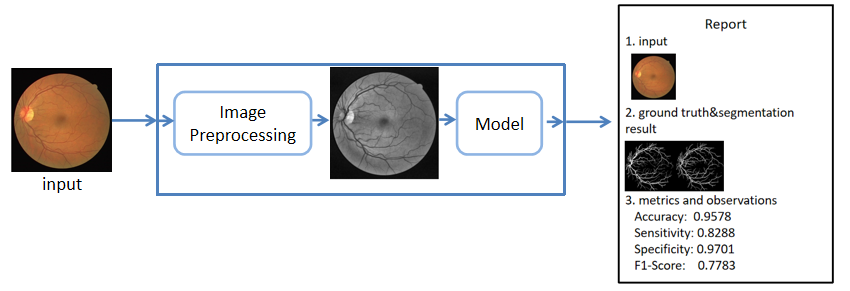
\includegraphics[width=0.80\textwidth]{overview}
\caption{Overview of RVSS}
\label{Fig_overview} 
\end{center}
\end{figure}


\subsubsection{Image Preprocessing Test}
\label{image_preprocessing}
During the acquisition process of fundus images, they are often affected by external conditions, causing uneven grayscale distribution in the acquired images. In addition, the contrast between the retinal image blood vessels and the background is low, making the retinal blood vessels difficult to detect (as shown in Figure \ref{fundus}). The Image Preprocessing of the RVSS is important for ensuring that input fundus images are optimized for the subsequent vessel segmentation process. Effective image preprocessing improves the accuracy of the segmentation results by enhancing image quality and standardizing image features. The tests designed for this stage are tailored to verify that the preprocessing methods meet the functional requirements as outlined in the \href{https://github.com/lele0007/Blood-vessel-segmentation/blob/main/docs/SRS/SRS.pdf}{SRS} document.

\begin{figure}[h!]
\begin{center}
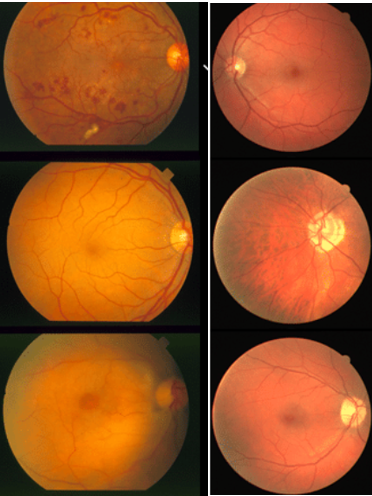
\includegraphics[width=0.20\textwidth]{fundus}
\caption{
Fundus images under different conditions.}
\label{fundus} 
\end{center}
\end{figure}


\begin{enumerate}

\item{test-image-preprocessing-id1: Image Upload and Format Validation \\}
\label{test-id-1}
Control: Automatic 
					
Initial State: The system is ready to receive fundus images as input. 
					
Input: Fundus images in various formats (JPEG, PNG, TIFF and an unsupported format, e.g., GIF), as shown in \autoref{tab:tc-image-1}
					
Output: Either give an appropriate message shows that the fundus image has been uploaded successfully and is accepted by the system (the input image is in JPEG, PNG or TIFF format) or give an error message shows that the image is rejected by the system (the input image is in an unsupported format.) 

Test Case Derivation: This test case is to test the behaviour of the system when the system is supplied with inputs for area that are the original fundus images. Based on the SRS document, the RVSS should accept commonly used and medically relevant image formats (JPEG, PNG, or TIFF). The rejection of unsupported formats ensures the system's processing capabilities are focused on compatible and clinically valuable fundus image data. In test cases TC-IMAGE-1-1 to TC-IMAGE-1-3, the system produces the Uploaded successfully message, and in test case TC-IMAGE-1-4, the system produces the Unsupported format message since it is an invalid input.    
					
How test will be performed: The automation script will attempt to upload images in each specified format (JPEG, PNG, and GIF format). The system responds to each uploaded image and compares it with the expected results.
\begin{center}
\begin{table}\centering
    \begin{tabular}{ lcccccc }    
    \hline
    \multicolumn{1}{c|}{ID} &     &   Input  &    &   \multicolumn{1}{c|}{}   &      &   Output    \\ \hline
    
    TC-IMAGE-1-1   &     &  01\underline{\hspace{0.5em}}test.tif &    &      &   & Uploaded successfully                    \\
    TC-IMAGE-1-2   &       & 02\underline{\hspace{0.5em}}test.png  &    &     &   & Uploaded successfully \\
    TC-IMAGE-1-3   &    & 03\underline{\hspace{0.5em}}test.jpeg  &   &     &    & Uploaded successfully\\
    TC-IMAGE-1-4   &    & 04\underline{\hspace{0.5em}}test.gif  &   &          &   & Unsupported format \\ 
    \hline    
   \end{tabular}  %
\caption{TC-IMAGE-1 - Image format input constraints tests}
\label{tab:tc-image-1}
\end{table}
\end{center}

\item{test-image-preprocessing-id2: Image Quality Preprocessing\\}
\label{test-id-2}
Control: Automatic 
					
Initial State: Fundus images in supported formats have uploaded successfully and are ready for preprocessing.
					
Input: Fundus images that vary in brightness, contrast, and presence of noise.
					
Output: Preprocessed images that exhibit standardized brightness and contrast levels appropriate for segmentation, with reduced noise while retaining critical details like vessel borders.

Test Case Derivation: This test case is to test the behaviour of the system when the system is supplied with inputs for area that are the original fundus images. This test case is to test the behaviour of the system on improving the quality of the raw retinal image. The expectation that preprocessing enhances image qualities conducive to segmentation is derived from the requirement for RVSS to optimize images for analysis without losing detail. This is important for ensuring that subsequent segmentation accurately identifies blood vessels.

How test will be performed: A set of raw fundus images will be processed through the system's preprocessing function. The output will be analyzed using image analysis software or simply observe to quantify changes in brightness, contrast, and noise levels. 
\end{enumerate}


\subsubsection{Vessel Segmentation Test}
\label{vessel_segmentation}
The vessel segmentation component is the core of the RVSS, tasked with accurately identifying and delineating the blood vessels within fundus images. The tests designed for this stage are tailored to verify that the segmentation methods meet the functional requirements as outlined in the \href{https://github.com/lele0007/Blood-vessel-segmentation/blob/main/docs/SRS/SRS.pdf}{SRS} document.

\begin{enumerate}

\item{test-vessel-segmentation-id3: Segmentation Image\\}
\label{test-id-3}
Control: Automatic 
					
Initial State: The system has loaded the pre-trained segmentation model and is ready to receive retinal images.
					
Input: Network pre-trained model parameters obtained from different rounds of training, fundus images and corresponding ground truth images with manually annotated blood vessels.
					
Output: Segmented images where the retinal vessels are identified and delineated.

Test Case Derivation: This test case is to test the behaviour of the system when the system is supplied with inputs for area that are the preprocessed fundus images. Based on the SRS document, the RVSS should output corresponding segmentation images, which are marked in binary format (e.g., vessels as 1, background as 0).
					
How test will be performed: The automation script will attempt to upload different network pre-trained model parameters and images into the RVSS and collecting the output segmented images.



\end{enumerate}


\subsubsection{Report Generation Test}
\label{report_generation}
The report of the RVSS includes the segmentation outcomes and metrics (e.g., accuracy, sensitivity, specificity). The tests designed for this stage are tailored to verify that the segmentation methods meet the functional requirements as outlined in the \href{https://github.com/lele0007/Blood-vessel-segmentation/blob/main/docs/SRS/SRS.pdf}{SRS} document.

\begin{enumerate}

\item{test-report-generation-id4: Report Generation\\}
\label{test-id-4}
Control: Manual 
					
Initial State: Segmentation analysis of various retinal images is available for report generation.
					
Input:  Fundus image, output of the segmentation algorithm (i.e., segmentation images which are marked in binary format), and a range of metrics (e.g., accuracy, sensitivity, specificity).
					
Output: Reports that include all relevant metrics and observations from the segmentation analysis, leaving no important information unreported.

Test Case Derivation: The need for comprehensive reporting is justified by the system’s aim to provide a full overview of the segmentation analysis.
					
How test will be performed: The reports will include existing and commonly used analytical criteria to ensure that all necessary information is included and clearly presented.
\end{enumerate}


\subsection{Tests for Nonfunctional Requirements}

Nonfunctional requirements for the RVSS are given in \href{https://github.com/lele0007/Blood-vessel-segmentation/blob/main/docs/SRS/SRS.pdf}{SRS} section 5.2. There are five nonfunctional requirements the RVSS. 



\subsubsection{Nonfunctional: Accuracy}
\label{non_functional_accuracy}		
The accuracy in the RVSS are critical for ensuring the outputs of the system are reliable and trustworthy. 

\begin{enumerate}

\item{test-id5: Accuracy Test\\}
\label{test-id-5}
Type: Automatic
					
Initial State: The system has completed the segmentation of retinal vessels from the fundus image.
					
Input: The segmentation result and the images of manually annotated blood vessels by experts (ground truth).
					
Output: The accuracy of the segmentation result. 
					
How test will be performed: The test will be performed by feeding the input images into the RVSS and collecting the output segmented images. The segmentation images will be compared against the ground truth using accuracy. Automated tools will calculate these accuracy. In addition, for unlabeled data, we can manually mark it, draw corresponding blood vessel segmentation images, and then analyze the model accuracy.
\end{enumerate}


\subsubsection{Nonfunctional: Robustness}
\label{non_functional_Robustness}		
Given the variability in real-world fundus images, the system must maintain high segmentation performance regardless of image quality or condition, as robustness is critical for ensuring the utility of the system in real settings. 

\begin{enumerate}

\item{test-id6: Robustness Test\\}
\label{test-id-6}
Type: Automatic
					
Initial State: The system is ready to process retinal images, with the pre-trained segmentation model loaded.
					
Input: Fundus images with various conditions, including low contrast, presence of noise, and varying lighting conditions.
					
Output: Segmented images where the retinal vessels are identified and delineated across all tested conditions, demonstrating the robustness of the algorithm.

How test will be performed: Each image will be processed through the pre-trained segmentation model. The segmentation images for each condition will be reviewed to assess robustness of the segmentation algorithm. Manual blood vessel annotation images (ground truth) from domain experts will be used to evaluate the segmentation results to ensure the effectiveness of the system under different image conditions.
\end{enumerate}



\subsubsection{Nonfunctional: Usability}
\label{non_functional_usability}	
Usability is a key nonfunctional requirement for the RVSS, affecting how easily healthcare professionals can interact with the system. Usability testing will involve direct user interaction with the system followed by feedback collection through surveys. 

\begin{enumerate}
					
\item{test-id7: Usability Test\\}
\label{test-id-7}
Type: Manual, Dynamic
					
Initial State: All features of the RVSS are accessible, including image upload, segmentation processing, and report generation functionalities. 
					
Input/Condition: 
\begin{itemize}
    \item Participant: volunteers recruited to test the system
    \item Materials: a set of fundus images for testing, tasks or scenarios designed to guide the participants through the system's functionalities, and a usability survey for feedback collection.
\end{itemize}
					
Output/Result: 
\begin{itemize}
    \item Quantitative Data: metrics such as task completion time, error rates during task execution, and frequency of help requests.
    \item Qualitative Data: Participant feedback on the system's ease of use, interface intuitiveness, satisfaction with the segmentation process time, and overall experience. This includes suggestions for improvements.
    \item Survey Responses: Structured responses collected through the usability survey, addressing specific aspects of system usability and user satisfaction.
\end{itemize}

How test will be performed: 
\begin{itemize}
    \item Preparation: recruit volunteers, prepare a set of predefined tasks (section \ref{7_1}) that cover the key functionalities of the system, designed to simulate typical use cases, and develop a usability survey (section \ref{7_2}) that includes questions on ease of use, interface design, functionality satisfaction, and overall user experience.
    \item Execution: conduct a briefing session for participants to explain the purpose of the test and provide basic instructions on using the system, then let  participants complete the predefined tasks, and fill out the usability survey, providing their feedback on the system.
\end{itemize}

\end{enumerate}


\subsubsection{Nonfunctional: Performance}
\label{non_functional_performance}	
The performance test for the RVSS is designed to evaluate the efficiency of the system, ensuring that it meets the non-functional requirements for processing speed under varying loads.

\begin{enumerate}					
\item{test-id8: Performance Test\\}
\label{test-id-8}
Type: Dynamic, Automatic
					
Initial State: The RVSS is running, ready to receive and process uploaded fundus images for vessel segmentation 
					
Input/Condition: A set of fundus images.
					
Output/Result: The time and resource utilization taken to process individual images and batches of images. 
					
How test will be performed: 
\begin{itemize}
    \item Preparation: select a representative set of fundus images for the test, and define performance benchmarks based on the requirements specified in the \href{https://github.com/lele0007/Blood-vessel-segmentation/blob/main/docs/SRS/SRS.pdf}{SRS} document, such as acceptable processing times for single images and image batches.
    \item Single Image Processing: upload an individual image to the system and measure the time and resource utilization taken from upload to the completion of the segmentation process, then record the processing time for each image and compare it against the predefined benchmarks.
    \item Batch Processing: upload batches of images, and measure the total time and resource utilization taken to process each batch.
    \item Draw graphs as shown in Figure \ref{graph})
\end{itemize}

\begin{figure}[h!]
\begin{center}
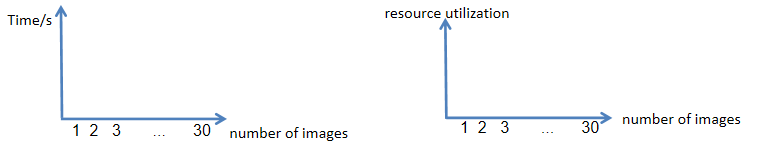
\includegraphics[width=0.70\textwidth]{graph}
\caption{
Performance Test graphs.}
\label{graph} 
\end{center}
\end{figure}

\end{enumerate}



\subsubsection{Nonfunctional: Compatibility}
\label{non_functional_compatibility}		
The compatibility test for the RVSS is designed to ensure 
the system is compatible with standard operating systems
used in healthcare environments.
\begin{enumerate}
					
\item{test-id9: Compatibility\\}
\label{test-id-9}
Type: Manual
					
Initial State: The RVSS is fully operational and configured for standard operations. 
					
Input: None 
					
Output: A report of what is running normally on the system or a log of any errors encountered.
					
How test will be performed: Install and run whole software in different operating systems. Also, need to ensure cases pass in all different operating system.
\end{enumerate}

\subsubsection{Nonfunctional: Maintainability}
\label{non_functional_maintainability}		
The maintainability test for the RVSS focuses on assessing the system's ease of modification, scalability, and adaptability to future requirements or technological advancements. 
\begin{enumerate}
					
\item{test-id10: Maintainability\\}
\label{test-id-10}
Type: Manual
					
Initial State: The RVSS code is in a stable state, with documentation, development environment setup, and version control system access ready. 
					
Input: The complete source code of RVSS, 
code for another segmentation network architecture to be replaced.
					
Output: The complete code of the system that network architecture has been replaced. 
					
How test will be performed: Modify the code based on predefined change requests (here replacing the segmentation network architecture is taken as an example) to simulate real maintainability scenarios.
\end{enumerate}

\subsection{Traceability Between Test Cases and Requirements}

A traceability between test cases and requirements is shown in \autoref{tab:tc-traceability}.

\begin{table}[h!]
\begin{center}
\begin{tabular}{ l|c|c|c|c|c|c|c|c|c }
\hline
 & R1   & R2 & R3 & R4  & NFR1 & NFR2 & NFR3 & NFR4 & NFR5 \\
\hline
\ref{image_preprocessing} & X & X & & & & & & \\
\hline
\ref{vessel_segmentation} &  & &X & & & & & \\
\hline
\ref{report_generation} & &  & &X & & & & \\
\hline
\ref{non_functional_accuracy} &  &  &X  & X & X & & & \\
\hline
\ref{non_functional_Robustness} &X  &  &  &  & X & & & \\
\hline	
\ref{non_functional_usability} & & & & & & X & & & \\
\hline
\ref{non_functional_performance} & & &X & & & & X & & \\
\hline
\ref{non_functional_compatibility} & & & & & & & & X & \\
\hline
\ref{non_functional_maintainability} & & & & & & & & & X \\

\hline
\end{tabular}
\caption{Tracebility between test cases and requirements}
\label{tab:tc-traceability}
\end{center}
\end{table}

\section{Unit Test Description}
\label{unit_test}
This section will be modified after finishing the design part.

The source code for the RVSS software has following modules, 
\begin{itemize}
    \item net.py - Provides network architecture for training. 
    \item data\_load.py - Loads and shows the raw fundus images. 
    \item data\_preprocess.py - Preprocesses fundus images .
    \item load\_params.py - Module for load the input parameters, including learning rate, training parameters, training data set, batch size, etc.
    \item train.py - Train the segmentation network using the training dataset. 
    \item test.py - Verifies the performance of the trained network using the test dataset.
    \item report.py - Generates a report including the segmentation outcomes and metrics values.
    
\end{itemize}

\subsection{Unit Testing Scope}
Unit testing is performed for the following modules: 

\begin{itemize}
    \item Load Data 
    \item Load Parameters
    \item Model Training
    \item Pretrained Model Testing
\end{itemize}
These modules are high priority modules that can affect the whole system if not work properly. Other modules like data preprocess and report modules are tested in the system as those have low priority static modules, so our system do not perform unit test on these module.  

\subsection{Tests for Functional Requirements} 

\subsubsection{Load Data Module (M1)}
A Load Data Module is assigned to loading fundus images in the folder with specified path.

\begin{enumerate}

\item{test-data-load-id11\\}
Type: Automatic
					
Initial State: The Load Data Module is initialized and ready to accept requests for loading data from specified sources.
					
Input/Condition: The path to the specified folder. 
					
Output/Result: Show all images in the folder.  
					
How test will be performed: Run the data\_load python file to check the correctness of the file.  

\end{enumerate}

\subsubsection{Load Parameters Module (M4)}
A Load Parameters Module is used to provide all parameters required for model training.

\begin{enumerate}

\item{test-parameter-load-id12\\}
Type: Automatic
					
Initial State: The Load Parameters Module includes all required parameters.
					
Input/Condition: N/A 
					
Output/Result: Pass, if parameters are loaded before model training.  
					
How test will be performed: Set the number of training epoch in the load\_params.py file to 0, and print the values of all parameters in the train.py file. If the printed parameter values are the same as the values set in load\_params.py file, the load\_params.py file is correct.  

\end{enumerate}


\subsubsection{Model Training Module (M5)}
A Model Training Parameters Module is used to train the segmentation model.

\begin{enumerate}

\item{test-model-train-id13\\}
Type: Automatic
					
Initial State: The Model Train Module is initialized.
					
Input/Condition: The training dataset. 
					
Output/Result: Output the value of each round of training process. For example, the output of the i-th round is ``Epoch i: loss value is 0.214".
					
How test will be performed: Run train.py and see the training log.  

\end{enumerate}

\subsubsection{Pretrained Model Testing (M6)}
A Pretrained Model Testing Module is used to test the performance of the pretrained segmentation network.

\begin{enumerate}

\item{test-model-test-id14\\}
Type: Automatic
					
Initial State: The Model Test Module is initialized.
					
Input/Condition: The test dataset. 
					
Output/Result: Output the corresponding segmentation result.
					
How test will be performed: Load the model weights obtained from train.py into test.py. Load the fundus images in the test dataset into the test.py file and output the segmentation results

\end{enumerate}


\subsection{Tests for Nonfunctional Requirements}
Unit testing the non-functional requirements is beyond the scope.

\subsection{Traceability Between Test Cases and Modules}
A traceability between test cases and modules is shown in \autoref{tab:tc-traceability-module} 

\begin{table}[h!]
\begin{center}
\begin{tabular}{ l|c|c|c|c|c|c }
\hline
 & M2  & M3 & M4 & M5 & M6 & M7   \\
\hline
test-image-preprocessing-id1 &X & & & & &   \\
\hline
test-image-preprocessing-id2 & &X & & & &  \\
\hline
test-vessel-segmentation-id3 & & & & &X &  \\
\hline
test-vessel-segmentation-id4 & & & X & X & X& \\
\hline
test-report-generation-id5 & & & & & &X  \\
\hline
test-data-load-id11 &X &  & & & & \\
\hline
test-parameter-load-id12 & & &X &X &  & \\
\hline
test-model-train-id13 & & &X &X &  &  \\
\hline
test-model-test-id14 &  & & &X &X & \\

\hline
\end{tabular}
\caption{Tracebility between test cases and module}
\label{tab:tc-traceability-module}
\end{center}
\end{table}



\section{Appendix}
\subsection{Predefined tasks in the usability test}
\label{7_1}
\textbf{Predefined tasks:}
\begin{itemize}
    \item[1.] Upload a Fundus Image
        \begin{itemize}
            \item[-]Select the option to upload a new fundus image.
            \item[-]Choose an image from the provided set and complete the upload process.
        \end{itemize}
    \item[2.] Initiate the segmentation process 
        \begin{itemize}
            \item[-]Initiate the vessel segmentation process for the uploaded image.
        \end{itemize}
    \item[3.] Review the segmentation image 
        \begin{itemize}
            \item[-]Access the completed segmentation results once the process is finished. 
            \item[-]Review the segmented image alongside the original, noting the delineation of retinal vessels.
        \end{itemize}
    \item[4.] Review the segmentation report
        \begin{itemize}
            \item[-] Use the option to review a report based on the segmentation results. 
            \item[-] Review the report within the system, noting the presentation and clarity of information.
        \end{itemize}
\end{itemize}



\subsection{User survey in the usability test}
\label{7_2}
\textbf{Usability Survey:}
\begin{itemize}
    \item Your role: 
      \begin{checklist}
        \item Medical researcher
        \item Segmentation algorithm researcher
        \item Others:
      \end{checklist}
    \item How familiar are you with medical image segmentation?
      \begin{checklist}
        \item Very Familiar
        \item Somewhat Familiar
        \item Not Familiar
      \end{checklist}
    \item How intuitive were the instructions for uploading and preparing images for segmentation?
      \begin{checklist}
        \item Very Intuitive
        \item Somewhat Intuitive
        \item  Neutral
        \item Somewhat Confusing
        \item  Very Confusing        
      \end{checklist}
    \item How would you rate the clarity of the segmentation results?
      \begin{checklist}
        \item Very Clear
        \item Clear
        \item  Neutral
        \item Somewhat Unclear 
        \item  Unclear      
      \end{checklist}
    \item How satisfied are you with the accuracy of the segmentation results?
      \begin{checklist}
        \item Very Satisfied
        \item Satisfied
        \item  Neutral
        \item Dissatisfied 
        \item  Very Dissatisfied       
      \end{checklist}
    \item What is the likelihood that the RVSS will be used in medical practice?
      \begin{checklist}
        \item Very Likely
        \item Likely
        \item  Neutral
        \item Unlikely 
        \item  Very Unlikely 
        \item Comments:
      \end{checklist}
    \item Does the system perform the segmentation tasks within an acceptable time?    
      \begin{checklist}
        \item Yes
        \item No
        \item  Comments:  
      \end{checklist}
    \item What features would you like to see improved or added to RVSS?   
      \begin{checklist}
        \item  Comments:  
      \end{checklist}



\end{itemize}


\bibliographystyle {plain}
\bibliography {ref}


\end{document}
